
  Our ultimate goal is to understand the relationship between liquidity constraints and precautionary saving. In this section we describe the relationship between consumption concavity and prudence; Kimball (\citeyear{kimball:smallandlarge}) shows that prudence induces precautionary saving, and below we that consumption concavity is induced by either liquidity constraints or precautionary saving.

  Our analysis of consumption concavity and prudence is couched in general terms and therefore applies whether the source of concavity is liquidity constraints or something else (e.g., uncertainty).\footnote{Another commonly employed source of concavity is an interest rate that smoothly increases as borrowing gets larger.}



\subsection{Definitions}
Our approach shows that the crucial question is whether the value function exhibits a property we call consumption concavity (CC). So we define property CC first, and then we define a \textit{counterclockwise concavification} which captures a specific class of transformations of a consumption function that make the modified function globally ``more'' concave.

\begin{defn}\label{defn:IntervalStrictCC} (Local Consumption Concavity.) \\ In relation to a
	utility function $u(c)$ with non-negative ($u''' \geq 0$) and non-increasing prudence, a function $V(w)$ has property CC (alternately, strict CC) over the
	interval between $w_{1}$ and $w_{2}$, where $w_2 >w_{1}$, if
	\[
	V'(w) = u'(c(w))
	\]
	for some increasing function $c(w)$ that satisfies concavity (alternately, strict concavity) over the interval from $w_{1}$ to $w_{2}$.
\end{defn}
Since (even with constraints) $V'(w) = u'(c(w))$ holds by the envelope theorem, $V(w)$ having property CC (alternately, strict CC) is the same as having a concave (alternately, strictly concave) consumption function $c(w)$.\footnote{Remember that the envelope theorem depends only on being able to spend \textit{current} wealth on \textit{current} consumption, so it holds whether or not there is a 	liquidity constraint.} Note that the definition is restricted to non-negative and non-increasing prudence. This encompasses most of the commonly used utility functions in the economics literature (e.g.\ CRRA, CARA, quadratic). Also, note that we allow for 'non-strict' concavity -- that is, linearity -- because we want to encompass cases such as quadratic utility in which parts of the consumption function can be linear.  Henceforth, unless otherwise noted, we will drop the cumbersome usage 'alternately, strict' -- the reader should assume that what we mean always applies in the two alternate cases in parallel.

If a function has property CC at every point, we define it as having property CC globally.
\begin{defn}\label{defn:PropCC} (Global Consumption Concavity.) \\  A function $V(w)$ has property CC in relation to a utility function $u(c)$ with $u'>0$, $u''<0$ if $V'(w) = u'(c(w))$ for some monotonically increasing concave function $c(w)$.
\end{defn}

We now show how consumption concavity affects the prudence of the value function. To compare two consumption functions and their respective concavity, we need to define when one function exhibits `greater' concavity than another.

\begin{defn}\label{defn:MoreCC} (Greater Consumption Concavity.) \\ Consider two functions $V(w)$ and $\hat{V}(w)$ that both exhibit property CC with respect to the same $u(c)$ at a point $w$ for some interval $(w_1,w_2)$ such that $w_1 < w < w_2$.  Then $\hat{V}(w)$ exhibits property `greater CC' compared to $V(w)$ if
	\begin{eqnarray}
	\hat{c}(w) - \left(\frac{w_{2}-w}{w_{2}-w_{1}} \hat{c}(w_{1})+\frac{w-w_{1}}{w_{2}-w_{1}}\hat{c}(w_{2})\right) \geq c(w) - \left(\frac{w_{2}-w}{w_{2}-w_{1}} c(w_{1})+\frac{w-w_{1}}{w_{2}-w_{1}}c(w_{2})\right) \label{eq:MoreCC}
	\end{eqnarray}
        cl	for all $w \in (w_{1},w_{2})$, and property `strictly' greater CC if \eqref{eq:MoreCC}
	holds as a strict inequality.
\end{defn}

If $c''$ and $\hat{c}''$ exist everywhere between $w_1$ and $w_2$, property CC is equivalent to $\hat{c}''$ being weakly larger in absolute value than $c''$ everywhere in the range from $w_1$ to $w_2$. The strict version of the proposition would require the inequality to hold strictly over some interval between $w_1$ and $w_2$.

The next concept we introduce is `counterclockwise concavification,' which describes an operation that makes the modified consumption function more concave than in the original situation. The idea is to think of the consumption function in the modified situation as being a twisted version of the consumption function in the baseline situation, where the kind of twisting allowed is a progressively larger increase in the MPC as the level of wealth gets lower. We call this a `counterclockwise concavification' to capture the sense that at any specific level of wealth, one can think of the increase in the MPC at lower levels of wealth as being a counterclockwise rotation of the lower portion of the consumption function around that level of wealth.

\begin{defn}\label{defn:cconcavification}(Counterclockwise Concavification.) \\
	Function $\hat{c}(w)$ is a counterclockwise concavification of $c(w)$ around $w^{\#}$ if the following conditions hold:
	\begin{enumerate}
		\item $\hat{c}(w) = c(w)$ for $w \geq w^{\#}$
		%\item $\lim_{\wAlt \downarrow w^{\#}}  \left(\frac{\hat{c}_{t}'(\wAlt)}{c_{t}'(\wAlt)}\right) = 1$
		\item $\lim_{w \uparrow w^{\#}} \left(\frac{\hat{c}'(w)}{c'(w)}\right)  \geq 1$
		\item $\lim_{\upsilon \uparrow w} \left(\frac{\hat{c}'(\upsilon)}{c'(\upsilon)}\right)$ is weakly decreasing in $w$ for $w \leq w^{\#}$
		\item If $\lim_{w \uparrow w^{\#}} \left(\frac{\hat{c}'(w)}{c'(w)}\right)  = 1$, then $\lim_{w \uparrow w^{\#}} \left(\frac{\hat{c}''(w)}{c''(w)}\right) > 1$
	\end{enumerate}
\end{defn}
The limits are necessary to allow for the possibility of discrete drops in the MPC at potential `kink points' in the consumption functions. To understand counterclockwise concavification, it is useful to derive its implied properties.


\begin{lemma}\label{lem:counterclockwise}(Properties of a Counterclockwise Concavification.) \\
	If $\hat{c}(w)$ is a counterclockwise concavification of $c(w)$ around $w^{\#}$ and $c''(w) \leq 0$ for all $w$, then
	\begin{enumerate}
		\item $\hat{c}(w) < c(w)$ for  $w < w^{\#}$.
		\item $\lim_{\upsilon \uparrow w} \hat{c}'(\upsilon) >$ $\lim_{\upsilon \uparrow w} c'(\upsilon)$ for $w < w^{\#}$.
		\item $\lim_{\upsilon \uparrow w} \hat{c}''(\upsilon) \leq \lim_{\upsilon \uparrow w} c''(\upsilon)$ for $w < w^{\#}$.
	\end{enumerate}
\end{lemma}
See Appendix \ref{app:counterclockwise} for the proof. A counterclockwise concavification thus reduces consumption, increases the MPC, and makes the consumption function more concave for all wealth levels below the point of concavification. Figure \ref{fig:counterclockwise} illustrates two examples of counterclockwise concavifications: the introduction of a constraint and the introduction of a risk. In both cases, we start from the situation with no risk or constraints (solid line). The introduction of a constraint is a counterclockwise concavification around a kink point $w^{\#}$. Below $w^{\#}$, consumption is lower and the MPC is greater. The introduction of a risk also generates a counterclockwise concavification of the original consumption function, but this time around $\infty$. For all $w < \infty$, consumption is lower, the MPC is higher, and the consumption function is strictly more concave.

\hypertarget{CounterclockwiseConcavifications}{}

\begin{figure}[ht]
	{\centering
	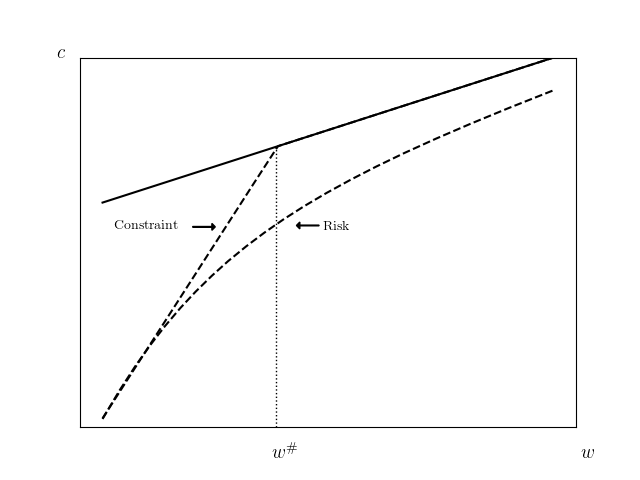
\includegraphics[width=.95\textwidth]{\FigDir/CounterclockwiseConcavifications}}
	\caption{Examples of Counterclockwise Concavifications}
	{\footnotesize \begin{singlespace} {\emph{Notes:} The solid line shows the linear consumption function in the case with no constraints and no risks. The two dashed line show the consumption function when we introduce a constraint and a risk, respectively. The introduction of a constraint is a counterclockwise concavification of the solid consumption function around $w^{\#}$, while the introduction of a risk is a counterclockwise concavification around $\infty$.}  \end{singlespace}}
	\label{fig:counterclockwise}
\end{figure}


\subsection{Consumption Concavity and Prudence}
The section above established all the tools necessary to show the relationship between consumption concavity and prudence. Our method in this section is to compare prudence in a \textit{baseline} case where the consumption function is $c(w)$ to prudence in a \textit{modified} situation in which the consumption function $\hat{c}(w)$ is a counterclockwise concavification of the baseline consumption function.

Our first result relates to the effects of a counterclockwise concavification on the absolute prudence of the value function.
\begin{defn}\label{defn:prudence}(Absolute Prudence of the Value Function.) \\
	Absolute prudence of the value function is defined as $-\frac{V'''(w)}{V''(w)}$.
\end{defn}

To understand the effects on prudence of a counterclockwise concavification, note that for a twice differentiable consumption function and thrice differentiable utility function, absolute prudence of the value function is defined as
\begin{equation} -\frac{V'''(w)}{V''(w)} = - \frac{u'''(c(w))}{u''(c(w))}c'(w) - \frac{c''(w)}{c'(w)} \label{eq:prudence}\end{equation}
by the envelope condition. The results we are about to derive in Theorem \ref{thm:CCToPrud} then follow easily. Theorem \ref{thm:CCToPrud} itself handles cases where the consumption function is not necessarily twice differentiable.
\begin{theorem}\label{thm:CCToPrud}  (Counterclockwise Concavification and Prudence.) \\
	Consider an agent who has a utility function %of the HARA class \eqref{eq:HARA}
	with $u' > 0$, $u'' < 0$, $u''' \geq 0$, and non-increasing absolute prudence ($-u'''/u''$). If $c(w)$ is concave and $\hat{c}(w)$ is a counterclockwise concavification of $c(w)$, then the value function associated with $\hat{c}(w)$ exhibits greater absolute prudence than the value function associated with $c(w)$ for all $w$.
\end{theorem}
\noindent See Appendix \ref{app:CCToPrud} for the proof.
There are three channels through which a counterclockwise concavification heightens prudence. First, the increase in consumption concavity from the counterclockwise concavification itself heightens prudence. Second, if the absolute prudence of the utility function is non-increasing, then the reduction in consumption (in some states) from the counterclockwise concavification makes agents more prudent at those states. And third, the higher marginal propensity to consume (MPC) from the counterclockwise concavification means that any given variation in wealth results in larger variation in consumption, increasing prudence. The channels operate separately, implying that a counterclockwise concavification heightens prudence \textit{even if absolute prudence is zero} as in the quadratic case.\footnote{cf.\ Nishiyama (\citeyear{nishiyama2012concavity})}
Theorem \ref{thm:CCToPrud} only provides conditions for when the value function exhibits greater prudence, but not \textit{strictly} greater prudence. In particular, the value function associated with $\hat{c}(w)$ will in some cases exhibit equal prudence for many values of $w$ and strictly greater prudence only for some values of $w$. In Corollary \ref{cor:ccandstrictprud}, we provide conditions for when the value function exhibits strictly greater prudence.
\begin{corollary} \label{cor:ccandstrictprud}(Counterclockwise Concavification and Strictly Greater Prudence.)\\
	Consider an agent who has a utility function with $u' > 0$, $u'' < 0$, $u''' \geq 0$, and non-increasing absolute prudence ($-u'''/u''$). If $c(w)$ is concave and $\hat{c}(w)$ is a counterclockwise concavification of $c(w)$ around $w^{\#}$, then the value function associated with $\hat{c}(w)$ exhibits strictly greater prudence than the value function associated with $c(w)$ if the utility function satisfies $u''' > 0$ and $w < w^{\#}$ or the utility function is quadratic ($u''' = 0$) and $\frac{\hat{c}'(w)}{c'(w)}$ strictly declines at $w$.
\end{corollary}
\noindent See Appendix \ref{app:ccandstrictprud} for the proof. For prudent agents ($u''' > 0$), the value function exhibits strictly greater prudence for all levels of wealth where the counterclockwise concavification affects consumption. This is because a reduction in consumption and higher marginal propensity to consume heighten prudence if the utility function has a positive third derivative and prudence is non-increasing. If the utility function instead is quadratic, the third derivative is zero and the absolute prudence of the utility function does not depend on the level of consumption or the marginal propensity to consume. In this case, the counterclockwise concavification only affects prudence at the kink points in the consumption function, i.e. where $\frac{\hat{c}'(w)}{c'(w)}$ strictly declines at $w$.
